% !TEX root = ../main.tex

\chapter{Evaluation}
\label{ch:evaluation}

\startcontents[chapters]

\vfill

\begin{alltt}\sffamily
Score,
quel grade avais,
of my cooler judgment,
and inquires after the evacuations of the toad on the horizon.

His judgment takes the winding way Of question distant,
if not always with judgment,
and showed him every mark of honour,
three score years before.

Designates him as above the grade of the common sailor,
but I was of a superior grade,
travellers of those dreary regions marking the site of degraded Babylon.

Mark the Quilt on which you lie,
und da Sie grade kein weißes Papier bei sich hatten,
and to draw a judgement from Heaven upon you for the Injustice.
\end{alltt}

\newpage
\minicontents
\spirals

\section{Evaluating Search}
\label{s:evalsearch}

Generally, computer systems are evaluated against functional requirements and performance specifications. Traditional \acf{IR} however is usually evaluated using two metrics known as precision and recall \autocite{Baeza-Yates2011}. Precision is defined as the fraction of retrieved documents that are relevant, while recall is defined as the fraction of relevant documents that are retrieved.

\begin{equation}
  Precision = \frac{\text{relevant documents retrieved}}{\text{retrieved documents}}
  \label{eq:precision}
\end{equation}
% \myequations{precision}

\begin{equation}
  Recall = \frac{\text{relevant documents retrieved}}{\text{relevant documents}}
\label{eq:recall}
\end{equation}
% \myequations{recall}

Note the slight difference between the two. Precision tells us how many of all retrieved results were actually relevant (of course this should preferable be very high) and recall simply indicates how many of all possible relevant documents we managed to retrieve. This can be easily visualised\sidepar{\faicon{object-group}~\ref{fig:PR}} as as shown in figure~\ref{fig:PR}.

\begin{figure}[!htbp]
  \centering
  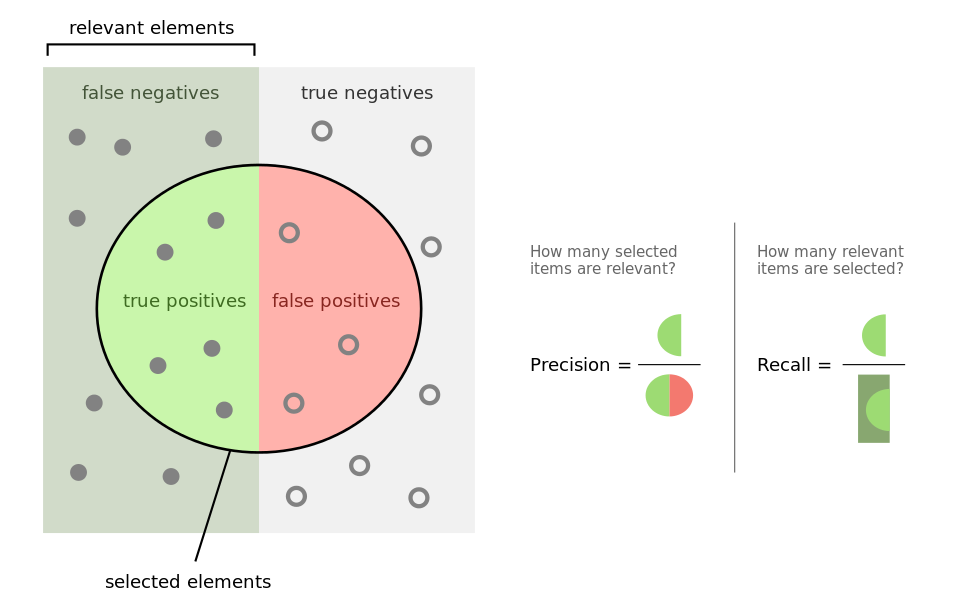
\includegraphics[width=\textwidth]{PRside}
  \caption[Precision and recall]{Precision and recall \autocite{Wikimedia2014}}
\label{fig:PR}
\end{figure}

Precision is typically more important than recall in web search, so often evaluation is reduced to measuring the \acf{MAP} value, which can be calculated using the formula in equation~\ref{eq:MAP}\sidepar{$\bm{\Sigma}$~\ref{eq:MAP}} \autocite{Baeza-Yates2011}, where $R_i$ is the set of results for query $i$, $P(R_i[k])$ is the precision value for result $k$ for query $i$ and $|R_i|$ is the total number of results.

\begin{equation}
  MAP_i = \frac{1}{|R_i|} \sum_{k=1}^{|R_i|} P(R_i[k])
\label{eq:MAP}
\end{equation}
% \myequations{MAP}

But for many web searches ii is not necessary to calculate the average of all results, since users don't inspect results after the first page very often and it is therefore desirable to have the highest level of precision in the first page of results maybe. For this purpose it is common to measure the average precision of web search engines after only a few documents have been seen. This is called `Precision at n' or `P@n' \autocite{Baeza-Yates2011}. So for example this could be P@5, P@10, or P@20. To compare two ranking algorithms, we would calculate P@10 for each of them over an average of 100 queries maybe and compare the results and therefore the performance of the algorithm.

The \acf{TREC} \autocite{Nist2016} provides large test sets of data \autocite{Trec2011} to participants and let's them compare results. They have specific test sets for web search comprised of crawls of $.gov$ web pages.

There are certain other factors that can be or should be evaluated when looking at a complete search system, as shown below \autocite{Baeza-Yates2011}. 

\begin{itemize}
  \item Speed of crawling.
  \item Speed of indexing data.
  \item Amount of storage needed for data.
  \item Speed of query response.
  \item Amount of queries per given time period.
\end{itemize}

Ranking is another issue that could be considered to pre-evaluate web pages at indexing time rather than query time. This was previously discussed in chapter~\ref{s:ranking}\sidepar{§~\ref{s:ranking}}.

\spirals

Evaluating creative search is more complex, as the notion of `relevance' is very different and this will be addressed in chapter~\ref{ch:interpretation}\sidepar{§~\ref{ch:interpretation}}. 

Sawle, Raczinski and Yang \autocite*{Sawle2011} discussed an initial approach to measure the creativity of search results in 2011. Based on a definition of creativity by Boden (as explained in chapter~\ref{s:boden}\sidepar{§~\ref{s:boden}}), we attempted to define creativity in a way which could be applied to search results and provide a simple metric to measure it. A copy of this paper can be found in appendix~\ref{app:pub}\sidepar{§~\ref{app:pub}}.


\section{Evaluating Creative Computers}
\label{s:creattributes}

This section moves on from evaluating search and focuses on evaluating creativity in computers.

\begin{quotation}
  The evaluation of artificial creative systems in the direct form currently practiced is not in itself empirically well-grounded, hindering the potential for incremental development in the field. \sourceatright{\autocite{Bown2014}}
\end{quotation}

Evaluating human creativity objectively seems problematic; evaluating computer creativity seems even harder. There are many debates across the disciplines involved. Taking theories on human creativity (see section~\ref{s:humancreativity}\sidepar{§~\ref{s:humancreativity}}) and directly applying them to machines (see section~\ref{s:compcreativity}\sidepar{§~\ref{s:compcreativity}}) seems logical but may be the wrong (anthropomorphic) approach\sidepar{§~\ref{ss:anthropomorphism}}. Adapting Mayer's five big questions \autocite*{Mayer1999} to machines does not seem to capture the real issues at play. Instead of asking if creativity is a property of people, products, or processes we might ask if it is a property of any or all of the following:

\begin{itemize}
  \item programmers
  \item users
  \item machines\footnote{This is problematic until the posited \ac{AI} singularity \autocite{Schmidhuber2006a}.}
  \item products
  \item processes
\end{itemize}

For instance, is the programmer the only creative agent, or are users (i.e. audiences or participants in interactive work) able to modify the system with their own creative input? Similarly for any instance of machine creativity, we might ask if it is:

\begin{itemize}
  \item local (e.g. limited to a single machine, program or agent)
  \item networked (i.e. interacts with other predefined machines or programs)
  \item web-based (e.g. is distributed and/or open to interactions, perhaps via an API)
\end{itemize}

Norton, Heath and Ventura highlight the importance of dealing with `evaluator bias' when using human judges for evaluating any form of creativity. They identified 5 main problems as follows \autocite*{Norton2015}. 

\begin{description}[leftmargin=3.5cm]
  \item[$1^{st}$ problem] Do we assess products or processes?
  \item[$2^{nd}$ problem] What are the measurable assessment criteria?
  \item[$3^{rd}$ problem] How do we un-ambiguate ambigous terminology?
  \item[$4^{th}$ problem] Which methodology to use for the assessment?
  \item[$5^{th}$ problem] How do we compensate for biases?
\end{description}

This point is also strengthend by Lamb, Brown and Clarke, saying that ``non-expert judges are very poor at using metrics to evaluate creativity'' and that the criteria they tested were not ``objective enough to produce trustworthy judgments'' \autocite*{Lamb2015}.


\subsection{Output minus Input}
\label{s:o-i}

Discussions from computational creativity often focus on very basic questions such as ``whether an idea or artefact is valuable or not, and whether a system is acting creatively or not'' \autocite{Pease2011}. Certain defining aspects of creativity, such as novelty and value (as discussed in chapter~\ref{ch:creativity}\sidepar{§~\ref{ch:creativity}}), are often used to measure the outcome of a creative process. These are highlighted throughout the following pages and further addressed in chapter~\ref{ch:interpretation}\sidepar{§~\ref{ch:interpretation}}.
 
One recurring theme is the clear separation of training data input and creative output in computers. Pease, Winterstein and Colton called this principle ``output minus input'' \autocite*{Pease2001}. The output in this case is the creative product but the input is not the process. Rather, it is the `inspiring set' (comprised of explicit knowledge such as a database of information and implicit knowledge input by a programmer) or training data of a piece of software.

\begin{quotation}
  The degree of creativity in a program is partly determined by the number of novel items of value it produces. Therefore we are interested in the set of valuable items produced by the program which exclude those in the inspiring set. \sourceatright{\autocite{Colton2001}}
\end{quotation}

They also suggest that all creative products must be ``novel and valuable'' \autocite{Pease2001} and provide several measures that take into consideration the context, complexity, archetype, surprise, perceived novelty, emotional response and aim of a product. In terms of the creative process itself they only discuss randomness as a measurable approach. Elsewhere, Pease et al discuss using serendipity as an approach \autocite*{Pease2013}.

Graeme Ritchie supports the view that creativity in a computer system must be measured ``relative to its initial state of knowledge'' \autocite*{Ritchie2007}. He identifies three main criteria for creativity as ``novelty, quality and typicality'' \autocite*{Ritchie2007}, although he argues that ``novelty and typicality may well be related, since high novelty may raise questions about, or suggest a low value for, typicality'' \autocite*{Ritchie2001,Ritchie2007}. He proposes several evaluation criteria which fall under the following categories \autocite*{Ritchie2007}: basic success, unrestrained quality, conventional skill, unconventional skill, avoiding replication and various combinations of those. Dan Ventura later suggested the addition of ``variety and efficiency'' to Ritchie's model \autocite*{Ventura2008}.

It should be noted that `output minus input' might easily be misinterpreted as `product minus process', however, that is not the case. In fact, Pease, Winterstein and Colton argue that ``the process by which an item has been generated and evaluated is intuitively relevant to attributions of creativity'' \autocite*{Pease2001}, and that ``two kinds of evaluation are relevant; the evaluation of the item, and evaluation of the processes used to generate it'' \autocite*{Pease2001}. If a machine simply copies an idea from its inspiring set then it just cannot be considered creative and needs to be disqualified so to speak.


\subsection{Creative Tripod}

Simon Colton came up with an evaluation framework called the \textit{creative tripod}. The tripod consists of three behaviours a system or artefact should exhibit in order to be called creative. The three legs represent ``skill, appreciation, and imagination'' and three different entities can sit on it, namely the programmer, the computer and the consumer. Colton argues that the perception ``that the software has been skillful, appreciative and imaginative, then, regardless of the behaviour of the consumer or programmer, the software should be considered creative'' \autocite*{Colton2008, Colton2008a}. As such a product can be considered creative, if it appears to be creative. If not all three behaviours are exhibited, however, it should not be considered creative \autocite{Colton2008, Colton2008a}.

\begin{quotation}
  Imagine an artist missing one of skill, appreciation or imagination. Without skill, they would never produce anything. Without appreciation, they would produce things which looked awful. Without imagination, everything they produced would look the same. \sourceatright{\autocite{Colton2008a}}
\end{quotation}

\spirals

Davide Piffer suggests that there are three dimensions of human creativity that can be measured, namely ``novelty, usefulness/appropriateness and impact/influence'' \autocite*{Piffer2012}. As an example of how this applies to measuring a person's creativity he proposes `citation counts' \autocite{Piffer2012}. While this idea works well for measuring scientific creativity maybe, he does not explain how this would apply to a visual artist for example.


\subsection{SPECS}
\label{s:specs}

Anna Jordanous proposed \num{14} key components of creativity (which she calls an ``ontology of creativity'') \autocite*{Jordanous2012}, from a linguistic analysis of creativity literature which identified words that appeared significantly more often in discussions of creativity compared to unrelated topics \autocite*{Jordanous2012}.

\begin{quotation}
  The themes identified in this linguistic analysis have collectively provided a clearer ``working'' understanding of creativity, in the form of components that collectively contribute to our understanding of what creativity is. Together these components act as building blocks for creativity, each contributing to the overall presence of creativity; individually they make creativity more tractable and easier to understand by breaking down this seemingly impenetrable concept into constituent parts. \sourceatright{\autocite{Jordanous2012}}
\end{quotation}

The 14 components Jordanous collated are: \autocite*{Jordanous2012}
\begin{quotation}
  \begin{enumerate}
    \item Active Involvement and Persistence
    \item Generation of Results
    \item Dealing with Uncertainty
    \item Domain Competence
    \item General Intellect
    \item Independence and Freedom
    \item Intention and Emotional Involvement
    \item Originality
    \item Progression and Development
    \item Social Interaction and Communication
    \item Spontaneity / Subconscious Processing
    \item Thinking and Evaluation
    \item Value
    \item Variety, Divergence and Experimentation
  \end{enumerate}
\end{quotation}

Jordanous also found that ``evaluation of computational creativity is not being performed in a systematic or standard way'' \autocite*{Jordanous2011} and proposed `\ac{SPECS}' \autocite*{Jordanous2012a}:

\begin{quotation}
  \begin{enumerate}
    \item Identify a definition of creativity that your system should satisfy to be considered creative:
      \begin{enumerate}
        \item What does it mean to be creative in a general context, independent of any domain specifics?
        \begin{itemize}
          \item Research and identify a definition of creativity that you feel offers the most suitable definition of creativity.
          \item The 14 components of creativity identified in Chapter 4 are strongly suggested as a collective definition of creativity.
        \end{itemize}
        \item What aspects of creativity are particularly important in the domain your system works in (and what aspects of creativity are less important in that domain)?
        \begin{itemize}
          \item Adapt the general definition of creativity from Step 1a so that it accurately reflects how creativity is manifested in the domain your system works in.
        \end{itemize}
      \end{enumerate}
    \item Using Step 1, clearly state what standards you use to evaluate the creativity of your system.
      \begin{itemize}
        \item Identify the criteria for creativity included in the definition from Step 1 (a and b) and extract them from the definition, expressing each criterion as a separate standard to be tested.
        \item If using Chapter 4's components of creativity, as is strongly recommended, then each component becomes one standard to be tested on the system.
      \end{itemize}
    \item Test your creative system against the standards stated in Step 2 and report the results.
      \begin{itemize}
        \item For each standard stated in Step 2, devise test(s) to evaluate the system's performance against that standard.
        \item The choice of tests to be used is left up to the choice of the individual researcher or research team.
        \item Consider the test results in terms of how important the associated aspect of creativity is in that domain, with more important aspects of creativity being given greater consideration than less important aspects. It is not necessary, however, to combine all the test results into one aggregate score of creativity.
      \end{itemize}
  \end{enumerate}
\end{quotation}

The \ac{SPECS} model essentially means that we cannot evaluate a creative computer system objectively, unless steps 1 and 2 are predefined and publically available for external assessors to execute step 3. Creative evaluation can therefore be seen as a move from subjectivity to objectivity, i.e. defining subjective criteria for objectively evaluating a product in terms of the initial criteria.

\begin{quotation}
  For transparent and repeatable evaluative practice, it is necessary to state clearly what standards are used for evaluation, both for appropriate evaluation of a single system and for comparison of multiple systems using common criteria. \sourceatright{\autocite{Jordanous2012a}}
\end{quotation}

This is further strengthened by Richard Mayer stating that we need a ``clearer definition of creativity'' \autocite*{Mayer1999} and Linda Candy arguing for ``criteria and measures [for evaluation] that are situated and domain specific'' \autocite*{Candy2012}.

Jordanous also defined 5 `meta-evaluation criteria' of correctness, usefulness, faithfulness as a model of creativity, usability of the methodology, and generality \autocite*{Jordanous2014}.


\subsection{MMCE}
\label{s:mmce}

Linda Candy draws inspiration for the evaluation of (interactive) creative computer systems from \ac{HCI}. The focus of evaluation in \ac{HCI} has been on usability, she says \autocite*{Candy2012}. She argues that in order to successfully evaluate an artefact, the practitioner needs to have ``the necessary information including constraints on the options under consideration'' \autocite*{Candy2012}.

Evaluation happens at every stage of the process (i.e. from design $\to$ implementation $\to$ operation). Some of the key aspects of evaluation Candy highlights are:

\begin{itemize}
  \item aesthetic appreciation
  \item audience engagement
  \item informed considerations
  \item reflective practice
\end{itemize}

She goes on to introduce the \ac{MMCE} (shown in figure~\ref{fig:mmce}\sidepar{\faicon{object-group}~\ref{fig:mmce}}) with four main elements of people, process, product and context \autocite*{Candy2012} similar to some of the models of creativity\sidepar{§~\ref{ch:creativity}} we have seen in chapter~\ref{ch:creativity}.

\begin{figure}[!htbp]
  \centering
  \begin{tikzpicture}%[node distance = 2cm and 7cm]

    % Mid circle
    \begin{pgfonlayer}{foreground}
    \fill[white] (0,0) circle [radius=0.75cm];
    \draw [->,thick] (0,0.75) to [out=0,in=90] (0.75,0);
    \draw [->,thick] (0.75,0) to [out=-90,in=0] (0,-0.75);
    \draw [->,thick] (0,-0.75) to [out=180,in=-90] (-0.75,0);
    \draw [->,thick] (-0.75,0) to [out=90,in=180] (0,0.75);
    \end{pgfonlayer}

    % North east
    \fill [fill=white,draw] (3.5,0.2) -- (0.2,0.2) -- (0.2,3.5) to [out=0,in=90] (3.5,0.2);
    \draw (1.5,1.5) node {Process};
    \begin{pgfonlayer}{background}
    \draw [rounded corners] (2,1) rectangle (7,4);
    \draw (4.5,2.5) node [node font=\tiny,align=right]{\textbf{Evaluation-2 How?}\\ Problem finding, solution oriented,\\ explanatory, systematic,\\ practice-based, opportunistic\\ empirical reflective,\\ rules, standards};
    \end{pgfonlayer}
    \draw (4.5,5) node [node font=\tiny,align=right]{\textbf{Interactions}\\ Working practices, interactive experiences};

    % South east
    \fill [fill=white,draw] (3.5,-0.2) -- (0.2,-0.2) -- (0.2,-3.5) to [out=0,in=-90] (3.5,-0.2);
    \draw (1.5,-1.5) node {Product};
    \begin{pgfonlayer}{background}
    \draw [rounded corners] (2,-1) rectangle (7,-4);
    \draw (5,-2.5) node [node font=\tiny, align=right]{\textbf{Evaluation-3 What?}\\ Novel, original, appropriate,\\ useful, surprising, flexible,\\ fluent, engaging};
    \end{pgfonlayer}
    \draw (4,-5) node [node font=\tiny,align=right]{\textbf{Outcomes}\\ Artifacts, installations, performances, exhibitions};

    % South west
    \fill [fill=white,draw] (-0.2,-3.5) -- (-0.2,-0.2) -- (-3.5,-0.2) to [out=-90,in=180] (-0.2,-3.5);
    \draw (-1.5,-1.5) node {Context};
    \begin{pgfonlayer}{background}
    \draw [rounded corners] (-2,-1) rectangle (-7,-4);
    \draw (-5,-2.5) node [node font=\tiny, align=left]{\textbf{Evaluation-4 Where?}\\ Studio, living laboratory,\\ public space, museum,\\ constraints, opportunities,\\ acceptability, leading edge};
    \end{pgfonlayer}
    \draw (-5.3,-5) node [node font=\tiny,align=left]{\textbf{Environment}\\ Resources, costs, tools, time};

    % North west
    \fill [fill=white,draw] (-0.2,3.5) -- (-0.2,0.2) -- (-3.5,0.2) to [out=90,in=180] (-0.2,3.5);
    \draw (-1.5,1.5) node {People};
    \begin{pgfonlayer}{background}
    \draw [rounded corners] (-2,1) rectangle (-7,4);
    \draw (-5,2.5) node [node font=\tiny, align=left]{\textbf{Evaluation-1 Who?}\\ Capability, characteristics,\\ track record, reputation,\\ impact, influence};
    \end{pgfonlayer}
    \draw (-4.5,5) node [node font=\tiny,align=left]{\textbf{Creators}\\ Artists, designers, participants, performers};
  \end{tikzpicture}
  \caption[Candy's MMCE]{Candy's Multi-dimensional Model of Creativity and Evaluation}
  \label{fig:mmce}
\end{figure}

She proposes the following values or criteria for measurement \autocite*{Candy2012}.

\begin{description}[leftmargin=1.8cm]
  \item [People] capabilities, characteristics, track record, reputation, impact, influence (profile, demographic, motivation, skills, experience, curiosity, commitment)
  \item [Process] problem finding, solution oriented, exploratory, systematic, practice-based, empirical, reflective, opportunistic, rules, standards (opportunistic, adventurous, curious, cautions, expert, knowledgeable, experienced)
  \item [Product] novel, original, appropriate, useful, surprising, flexible, fluent, engaging (immediate, engaging, enhancing, purposeful, exciting, disturbing)
  \item [Context] studio, living laboratory, public space, museum, constraints, opportunities, acceptability, leading edge (design quality, usable, convincing, adaptable, effective, innovative, transcendent)
\end{description}


\subsection{CSF}
\label{s:csf}

Geraint Wiggins introduced a formal notation and set of rules for the description, analysis and comparison of creative systems called \ac{CSF}\autocite*{Wiggins2006} which is largely based on Boden's theory of creativity \autocite*{Boden2003}\sidepar{§~\ref{s:boden}}. The framework uses three criteria for measuring creativity: ``relevance, acceptability and quality''. Graeme Ritchie then contributed to this framework with several revisions \autocite*{Ritchie2012}.

The \ac{CSF} provides a formal description for Boden's concepts of exploratory and transformational creativity. Wiggins's `R–transformation' and `T–transformation' is akin to Boden's `H-creativity' and `P-creativity' respectively. To enable the transition from exploratory to transformational creativity in his framework, Wiggins introduced meta-rules which allow us to redefine our conceptual space in a new way.

It is important to note here that the exploratory search in an \ac{IR} sense (as discussed in section~\ref{s:browsing}\sidepar{§~\ref{s:browsing}}) should not be mistaken with the topic at hand. Exploratory search (for a creative solution to a problem) in the Wiggins/Ritchie/Boden sense happens one step before transformational search. This means that we want to end up with transformational tools from this framework (rather than exploratory ones) to use in our exploratory web search system.

Ritchie described the \ac{CSF} as a set of initial concepts, which create `further concepts one after another, thus ``exploring the space''' but also argued that a search system would practically only go through a limited number of steps and therefore proposed some changes and additions to the framework \autocite*{Ritchie2012}. He summarised Wiggins' original \ac{CSF} as consisting of the following basic elements:

% \begin{conditions}
%   U & the universal set of concepts \\
%   L & the language for expressing the relevant mappings \\
%   R & a symbolic representation of the acceptability map \\
%   E & a symbolic representation of the quality mapping \\
%   T & a symbolic representation of the search mechanism \\
%   \[ \] & an interpreter for expressions like $R$ and $E$ \\
%   \langle , , \rangle & an interpreter for expressions like $T$
% \end{conditions}

\begin{enumerate}
	\item the universal set of concepts $U$,
	\item the language for expressing the relevant mappings $L$,
	\item a symbolic representation of the acceptability map $R$,
	\item a symbolic representation of the quality mapping $E$,
  \item a symbolic representation of the search mechanism $T$,
	\item an interpreter for expressions like 3 and 4 $[ \ ]$, and
	\item an interpreter for expressions like 5 $\langle \ , \ , \ \rangle$.
\end{enumerate}

This set of elements is described as the `object-level' (enabling exploratory search). The `meta-level' (enabling transformational search) has the same seven elements with one exception; the universal set of concepts $U$ contains concepts described at the object-level. This allows transformations to happen; concepts from the object-level are searched using criteria and mechanisms (elements 2 to 5) from the meta-level, giving rise to a new and different subset of concepts to those which an object-level search would have produced.

A typical search process would go as follows. We start with an initial set of concepts $C$ that represent our conceptual space and a query. We then explore $C$ and find any elements that match the query with a certain quality (norm and value criteria) in a given amount of iterations. This produces the object-level set of exploratory concepts (in Boden's sense) which we would call the traditional search results. To get creative results we would need to apply the meta-level search (Boden's transformational search) with slightly different quality criteria.

Wiggins explained various situations of creativity not taking place (uninspiration and aberration) in terms of his framework as shown below. For example, a system not finding any valuable concepts would be expressed as $[E](U) = 0$ (in Wiggins' original notation). While this approach seems counter-intuitive and impractical, it actually provides an interesting inspiration on how to formulate some of our pataphysical concepts in terms of the \ac{CSF} (see chapter~\ref{s:pataasp}\sidepar{§~\ref{s:pataasp}}).

\begin{description}[leftmargin=10cm]
  \item [Hopeless Uninspiration] $V_\alpha (X) = \emptyset$\\ valued set of concepts is empty
  \item [Conceptual Uninspiration] $V_\alpha (N_\alpha (X)) = \emptyset$\\ no accepted concepts are valuable
  \item [Generative Uninspiration] $elements(A) = \emptyset$\\ set of reachable concepts is empty
  \item [Aberration] $B$ is the set of reachable concepts not in $[N]_\alpha (X)$ and $B \neq \emptyset$\\ search goes outside normal boundaries
  \item [Perfect Aberration] $V_\alpha (B) = B$
  \item [Productive Aberration] $V_\alpha (B) \neq \emptyset$ and $V_\alpha (B) \neq B$
  \item [Pointless Aberration] $V_\alpha (B) = \emptyset$
\end{description}

The potential of these definitions of `uncreativity' is further explored in chapter~\ref{ch:future}\sidepar{§~\ref{ch:future}}.


\subsection{Individual Criteria}
\label{s:indcrit}

Many separate attempts exist at defining an evaluation model that focuses on a single criterion for creativity.

One such example is a model for evaluating the `interestingness' of computer generated plots \autocite{Perez2013}.

Another approach looks at ``quantifying surprise by projecting into the future'' \autocite{Maher2013}.

Bown looks at ``evaluation that is grounded in thinking about interaction design, and inspired by an anthropological understanding of human creative behaviour'' \autocite*{Bown2014}. He argues that ``systems may only be understood as creative by looking at their interaction with humans using appropriate methodological tools'' \autocite*{Bown2014}. He proposed the following methodology.

\begin{enumerate}
  \item The recognition and rigorous application of `soft science' methods wherever vague unoperationalised terms and interpretative language is used.
  \item An appropriate model of creativity in culture and art that includes the recognition of humans as `porous subjects', and the significant role played by generative creativity in the dynamics of artistic behaviour.
\end{enumerate}

Others argues that creativity can be measured by looking at the overall `unexpectedness' of an artefact \autocite{Kazjon2014}. 

McGregor, Wiggins and Purver introduce the idea of creativity as an ``intimation of dualism, with its inherent mental representations, is a thing that typical observers seek when evaluating creativity'' \autocite*{Mcgregor2014}.

Another attempt to evaluate computational creativity suggests that systems must go through a sequence of 4 phases ``in order to reach a level of creativity acceptable to a set of human judges'' \autocite{Negrete2014}. The phases are as follows.

\begin{enumerate}
  \item \textbf{Structure} is the basic architecture of a piece; it is what allows spectators to make out different parts of it, to analyze it to understand its main organization.
  \item \textbf{Plot} is the specialization scaffold of the structure to one purpose; it is the basis for narrative and the most detailed part of planned structure. It is upon plots that pieces are rendered.
  \item \textbf{Rendering} is a particular way in which the plot was developed and filled with detail in order to be delivered to the audience.
  \item \textbf{Remediation} is the transformation of a creative piece already rendered into another one, re-rendered, possibly into another media.
\end{enumerate}

Fran\c{c}a et al. propose a system called \textit{Regent-Dependent Creativity} (RDC) to address the ``lack of domain independent metrics'' and which combines ``the Bayesian Surprise and Synergy to measure novelty and value, respectively '' \autocite*{Franca2016}. 

This dependency relationship is defined by a pair $P(r; d)$ associated with a numeric value $v$, where $r$ is the regent (a feature that contributes to describing an artifact), $d$ is the dependent (it can change the state of an attribute), and $v$ is a value that represents the intensity of a specific pair in different contexts. 

\begin{quotation}
  For example, an artifact car can be described by a pair $p_i(color; blue)$, where blue changes the state of the attribute color. The same artifact could also be described by another pair $p_i(drive; home)$, where the dependent home connects a target to the action drive. \sourceatright{\autocite{Franca2016}}
\end{quotation}

Velde et al. have broken down creativity into 5 main clusters \autocite*{Velde2015}:

\begin{itemize}
  \item Original (originality)
  \item Emotion (emotional value)
  \item Novelty / innovation (innovative)
  \item Intelligence
  \item Skill (ability)
\end{itemize}






\stopcontents[chapters]
